% BEGIN PREAMBEL
\documentclass[9pt]{beamer}
\usepackage[british]{babel}
\usepackage[latin1]{inputenc}
\usepackage{multimedia}
\usepackage{amsmath,amsfonts,amssymb}
\usepackage{upgreek}
\usepackage{pgfpages}
\usepackage[version=3]{mhchem}
\usepackage{lmodern}
\usepackage{graphicx}
\usepackage{multicol}
\usepackage{xcolor}
\usepackage{wrapfig}
\usepackage{siunitx}
\newcommand{\as}{\\[14pt]}
\newcommand{\s}{\\[7pt]}
\newcommand{\is}{\\[2pt]}
\newcommand{\no}{\noindent}
\newcommand{\ka}{\hspace*{0.5cm}}
\newcommand{\ma}{\hspace*{1cm}}
\newcommand{\ga}{\hspace*{1.5cm}}
\newcommand{\li}{\left|}
\newcommand{\re}{\right|}
\newcommand{\const}{\text{const.}}
\newcommand{\z}{\text}
\newcommand{\terminal}[1]{\colorbox{black}{\textcolor{white}{{\fontfamily{phv}\selectfont \scriptsize{#1}}}}}
\newcommand{\plugin}[1]{\textit{\flq#1\frq}}
\usetheme{Boadilla}
\graphicspath{ {Pics/} }
\usecolortheme{beaver}
\useoutertheme{miniframes}
\beamertemplatenavigationsymbolsempty
\makeindex
\title[Analysis]{Discussion of the Pad Analysis}
\author[M. Reichmann]{Michael Reichmann}
\institute[\textbf{\textit{ETH}}\scalebox{.6}{\textit{Z\"{u}rich}}]{Swiss Federal Institute of Technology Zurich}
% END PREAMBEL
\begin{document}
% ============================
% BEGIN TITLE PAGE
% ============================
\begin{frame}
	\begin{center}
		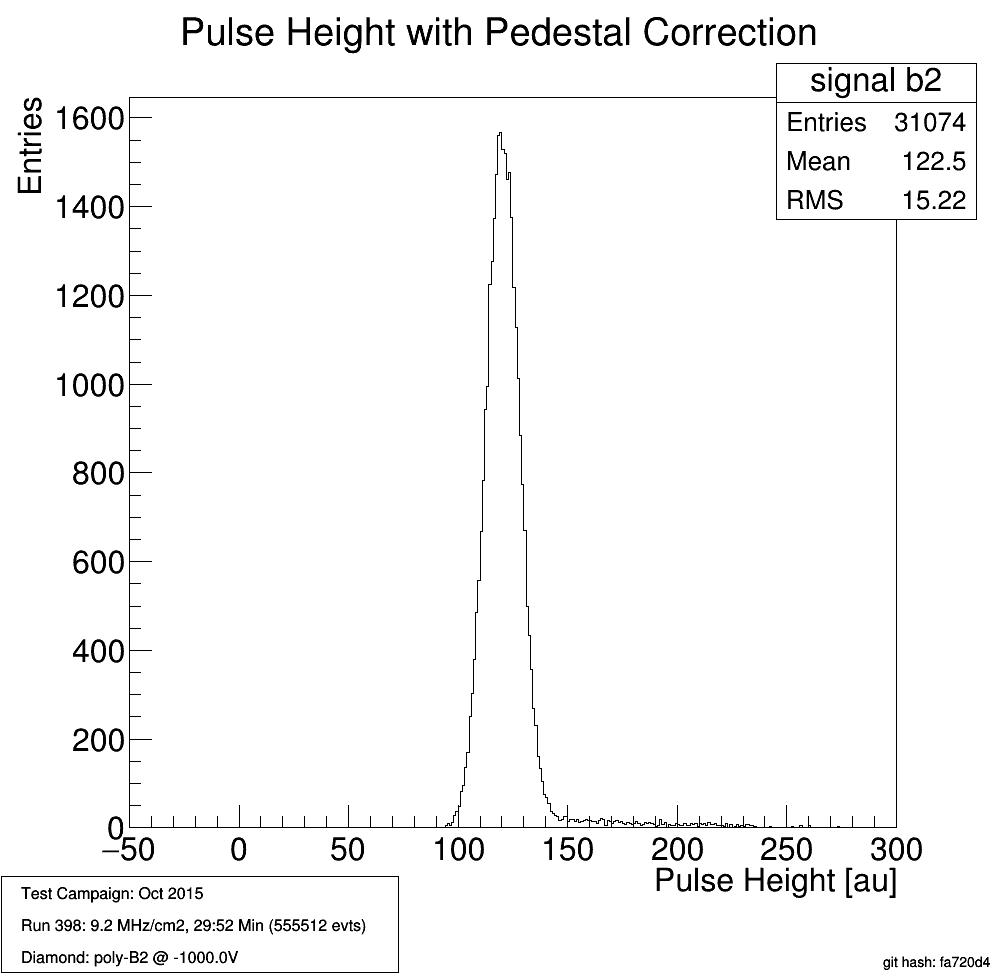
\includegraphics[width=6cm]{SignalDistribution}
	\end{center}
	\begin{alertblock}{
		\begin{center}
			\textbf{Meeting \today}
		\end{center}}
		\vspace*{10pt}
		\begin{center}\small
		Michael Reichmann
		\end{center}\normalsize
	\end{alertblock}
\end{frame}
% END
% ============================
% BEGIN TABLE OF CONTENTS
% ============================
\begin{frame}[allowframebreaks]
	\frametitle{Table of contents}
	\tableofcontents   % [pausesections]
\end{frame}
% END
% ====================================================================================
% PULSER
% ====================================================================================
\section{Pulser}
% ============================
\subsection{Waveforms}
\begin{frame}
	\frametitle{Waveforms}
	\begin{center}
		\begin{minipage}{5.5cm}
			\centering
			\textbf{\underline{External Pulser (S129)}}\s
			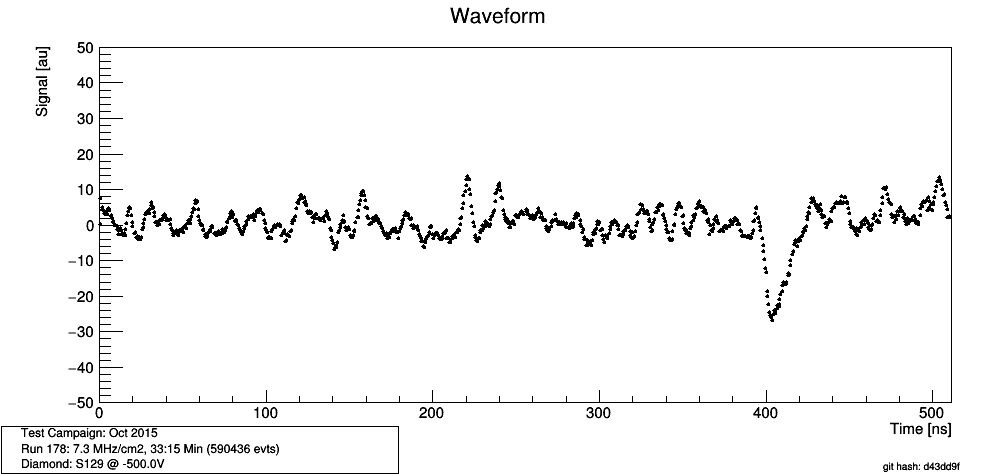
\includegraphics[width=5.5cm]{SingleWaveForm1}\\
			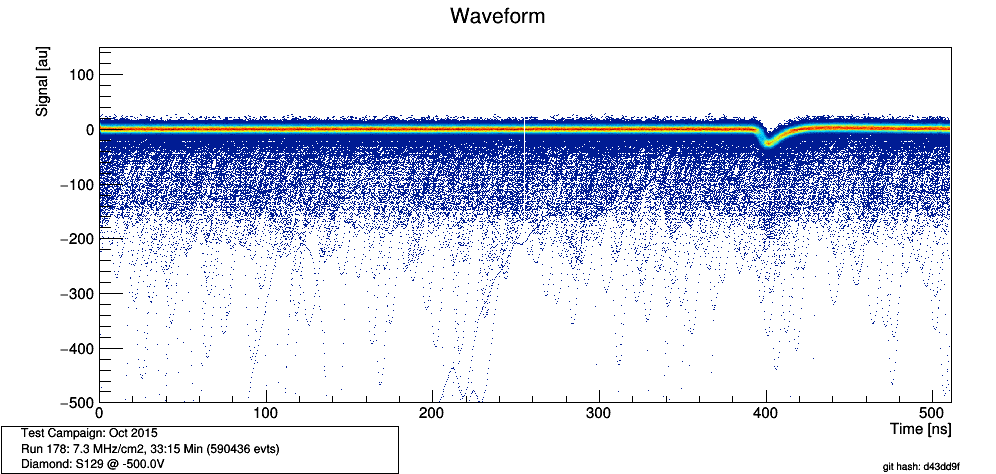
\includegraphics[width=5.5cm]{WaveForms50001}
		\end{minipage}
		\hspace*{2pt}
		\begin{minipage}{5.5cm}
			\centering
			\textbf{\underline{Internal Pulser (poly-B2)}}\s
			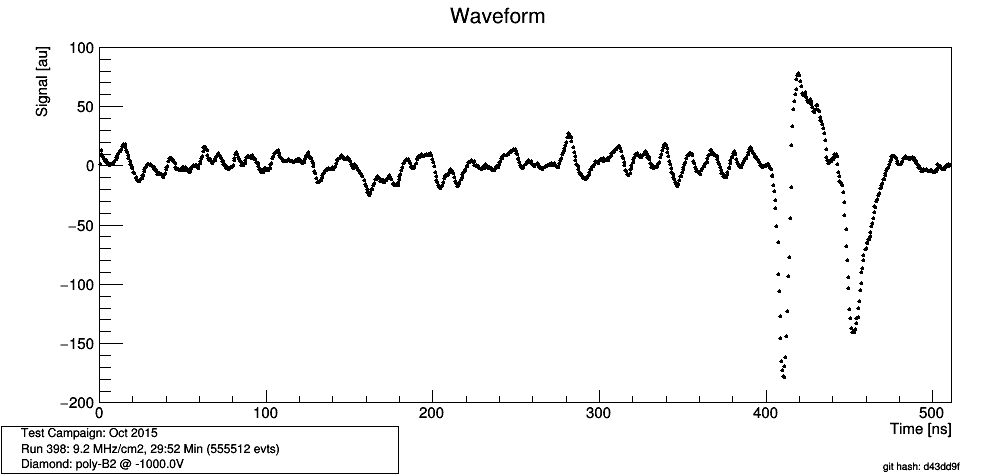
\includegraphics[width=5.5cm]{SingleWaveForm}\\
			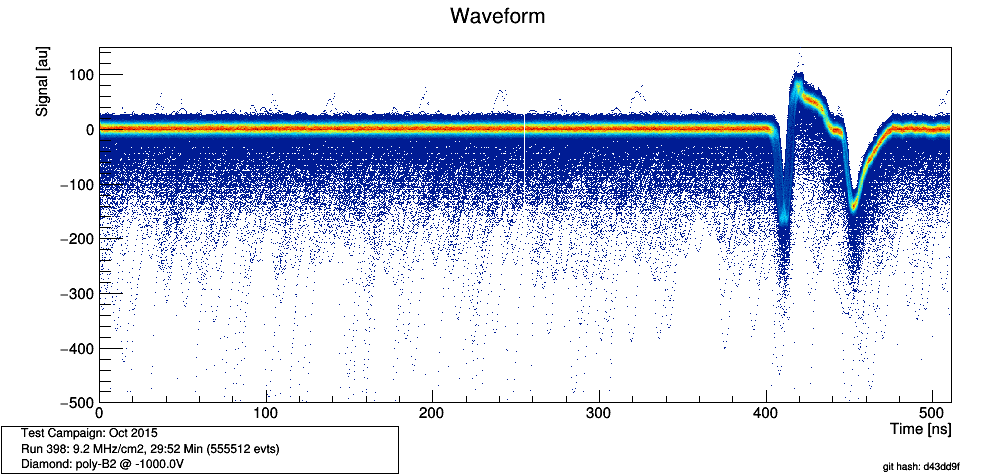
\includegraphics[width=5.5cm]{WaveForms5000}
		\end{minipage}\no\s
	\end{center}
\end{frame}
% ============================
\subsection{Distributions}
\begin{frame}
	\frametitle{Distribution Cuts}
	\underline{\textbf{Used Cuts:}}
	\begin{itemize}
		\setlength{\itemsep}{\fill}
		\item Pedestal Sigma: correct for base line shifts
		\item saturated Events: will most certainly influence pulser signal 
		\item Event Range: use the same event range (exclude first 5 min)
		\item Pulser
	\end{itemize}
	\vspace*{10pt}
	\underline{\textbf{Irrelevant Cuts:}}
	\begin{itemize}
		\setlength{\itemsep}{\fill}
		\item tracks, chi2, track-angle
		\item bucket
	\end{itemize}
	\vspace*{10pt}
	\underline{\textbf{Varying Cuts:}}
	\begin{itemize}
		\setlength{\itemsep}{\fill}
		\item beam interruptions
	\end{itemize}
\end{frame}
% new frame ============================
\begin{frame}
	\frametitle{Distributions}
	\begin{center}
		\begin{minipage}{3.5cm}
			\centering
			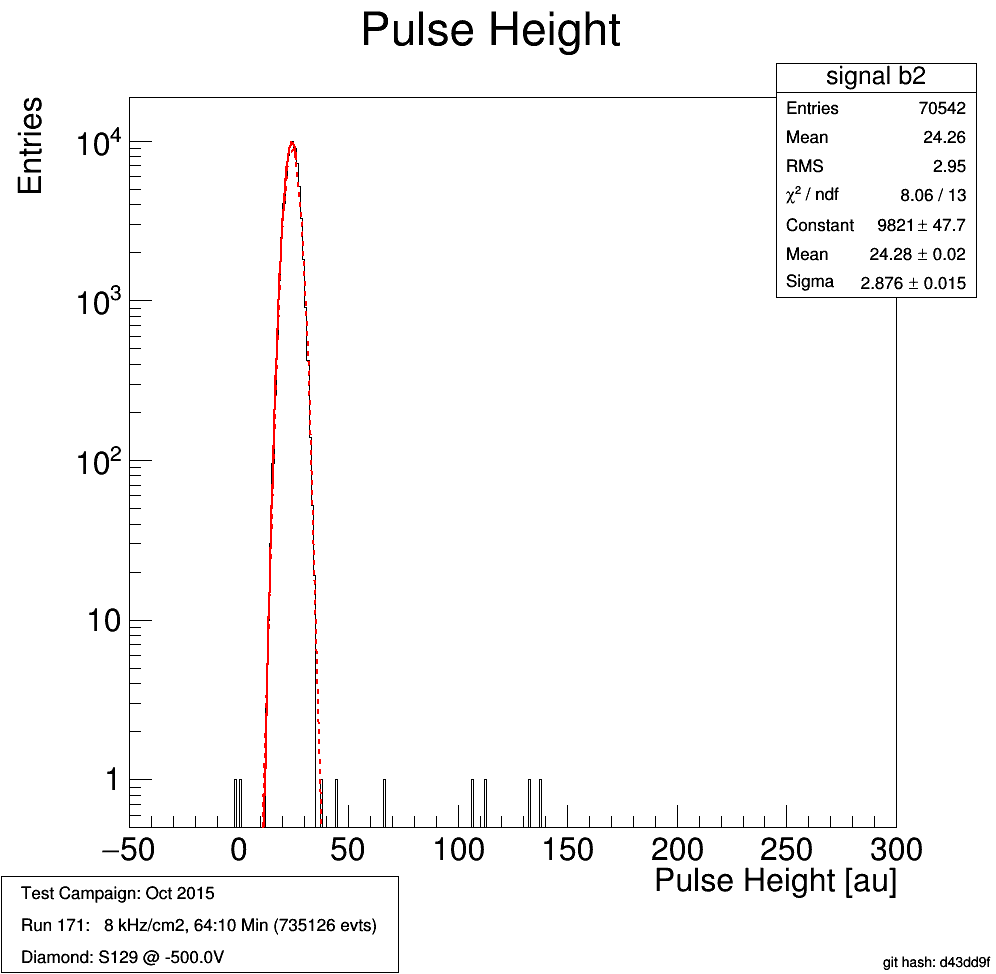
\includegraphics[width=3.45cm]{PulserHisto0}\\
			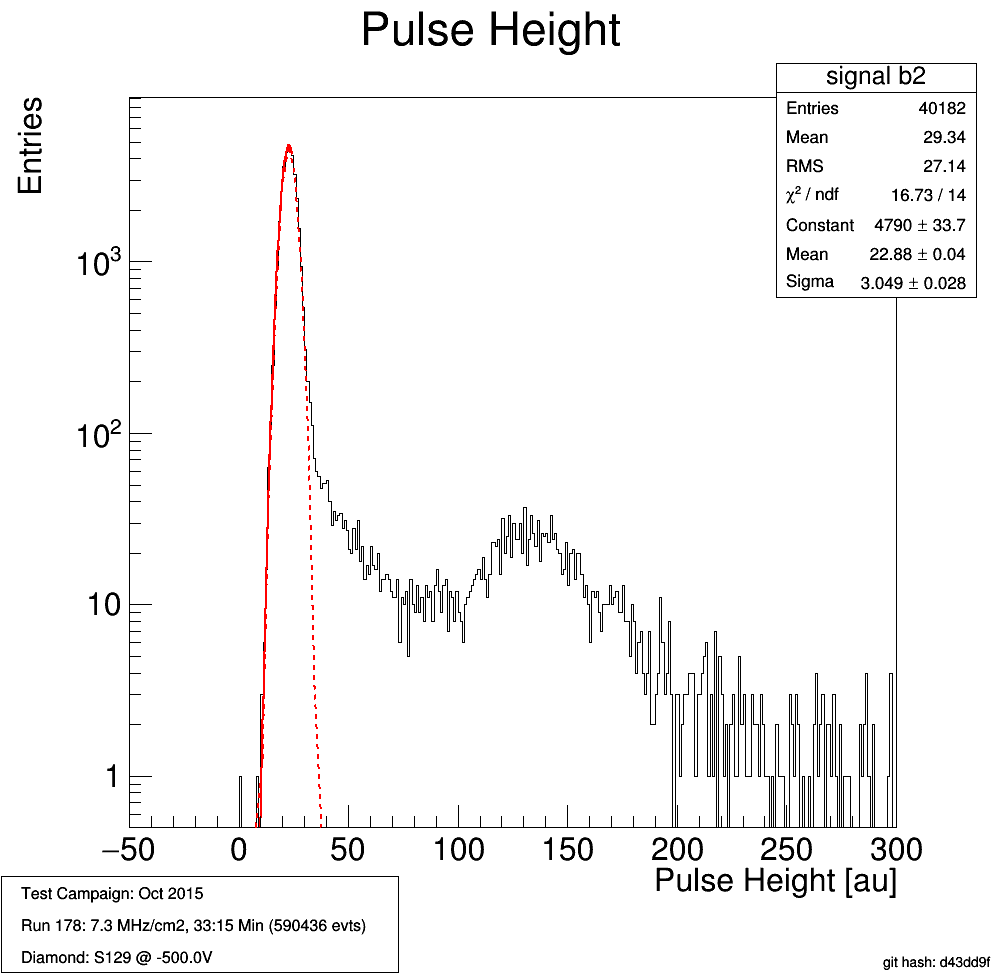
\includegraphics[width=3.45cm]{PulserHisto1}
		\end{minipage}
		\begin{minipage}{3.5cm}
			\centering
			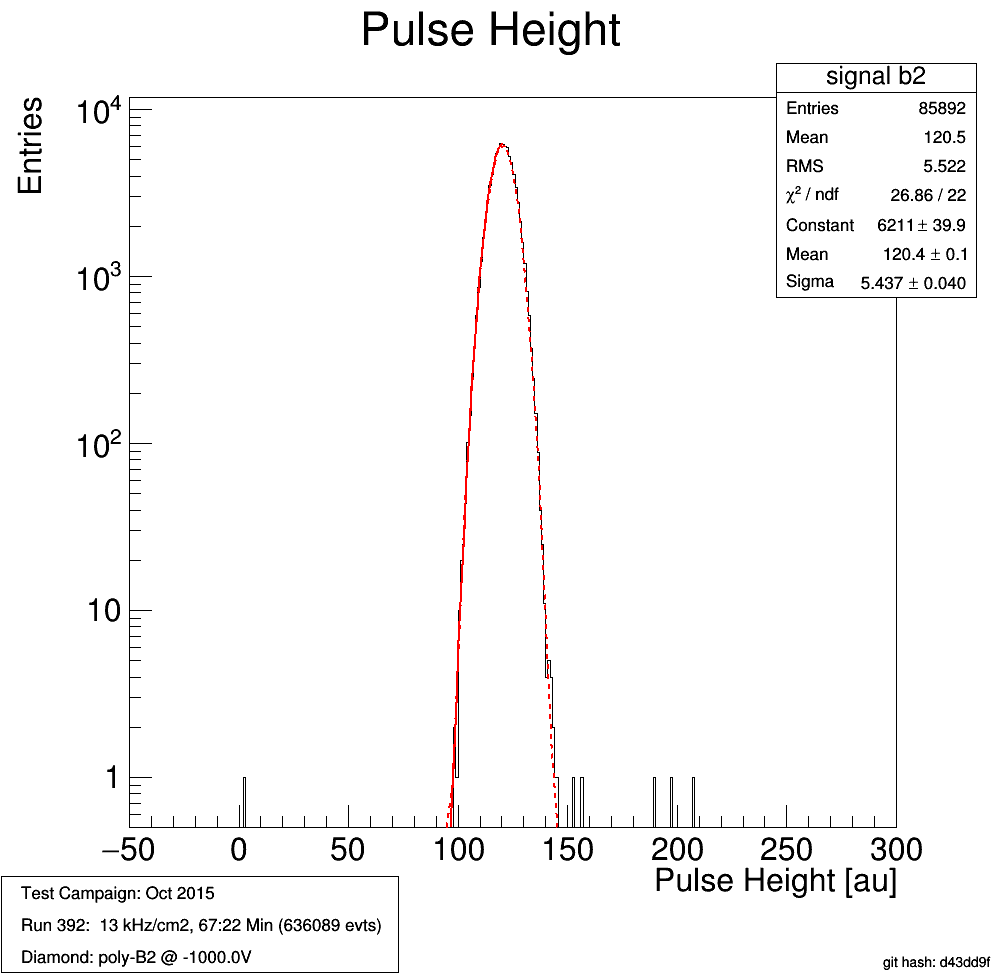
\includegraphics[width=3.45cm]{PulserHisto2}\\
			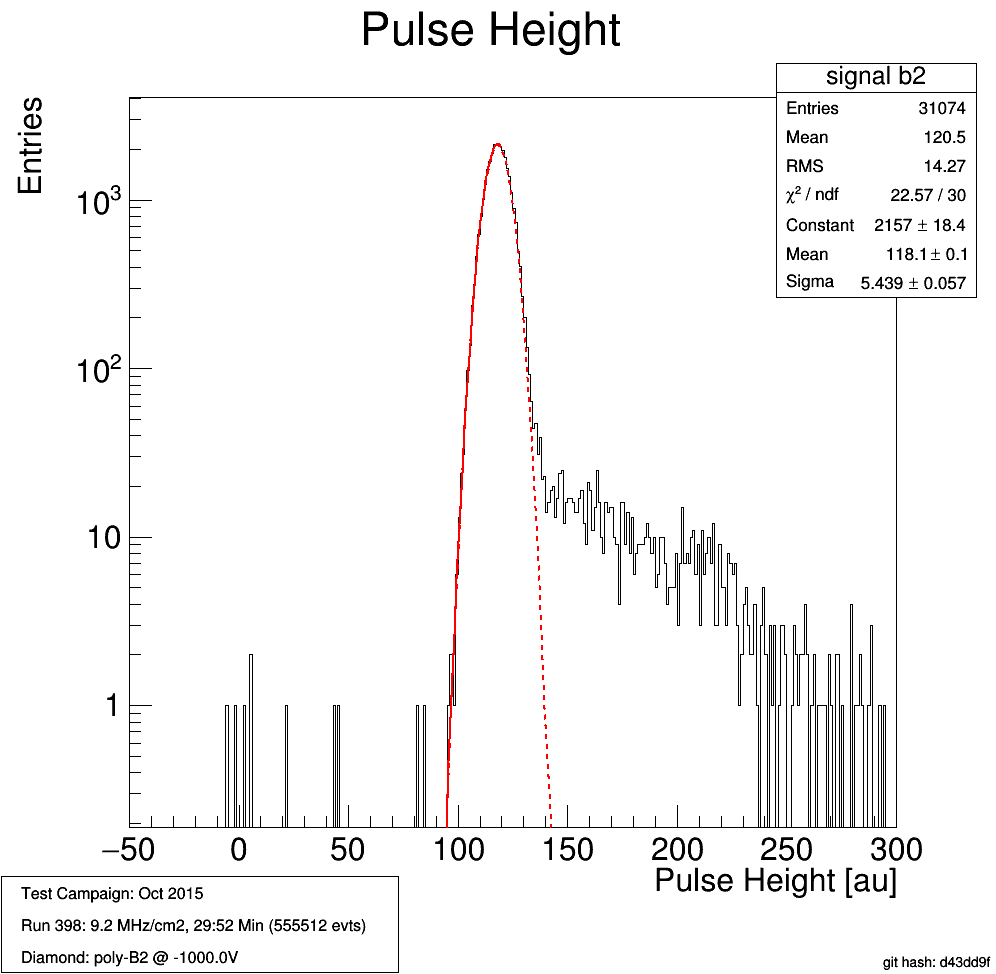
\includegraphics[width=3.45cm]{PulserHisto3}
		\end{minipage}
		\begin{minipage}[c][.5\textheight]{4cm}
			\begin{itemize}
				\setlength{\itemsep}{\fill}	
				\item fit only left side of the gaussian (least corrupted by signal)
				\item pedestal correction: substraction of the mean of the pedestal fit
			\end{itemize}
		\end{minipage}
	\end{center}
\end{frame}
% ============================
\subsection{Rate Dependence}
\begin{frame}
	\frametitle{II6B2 neg}
	\begin{center}
		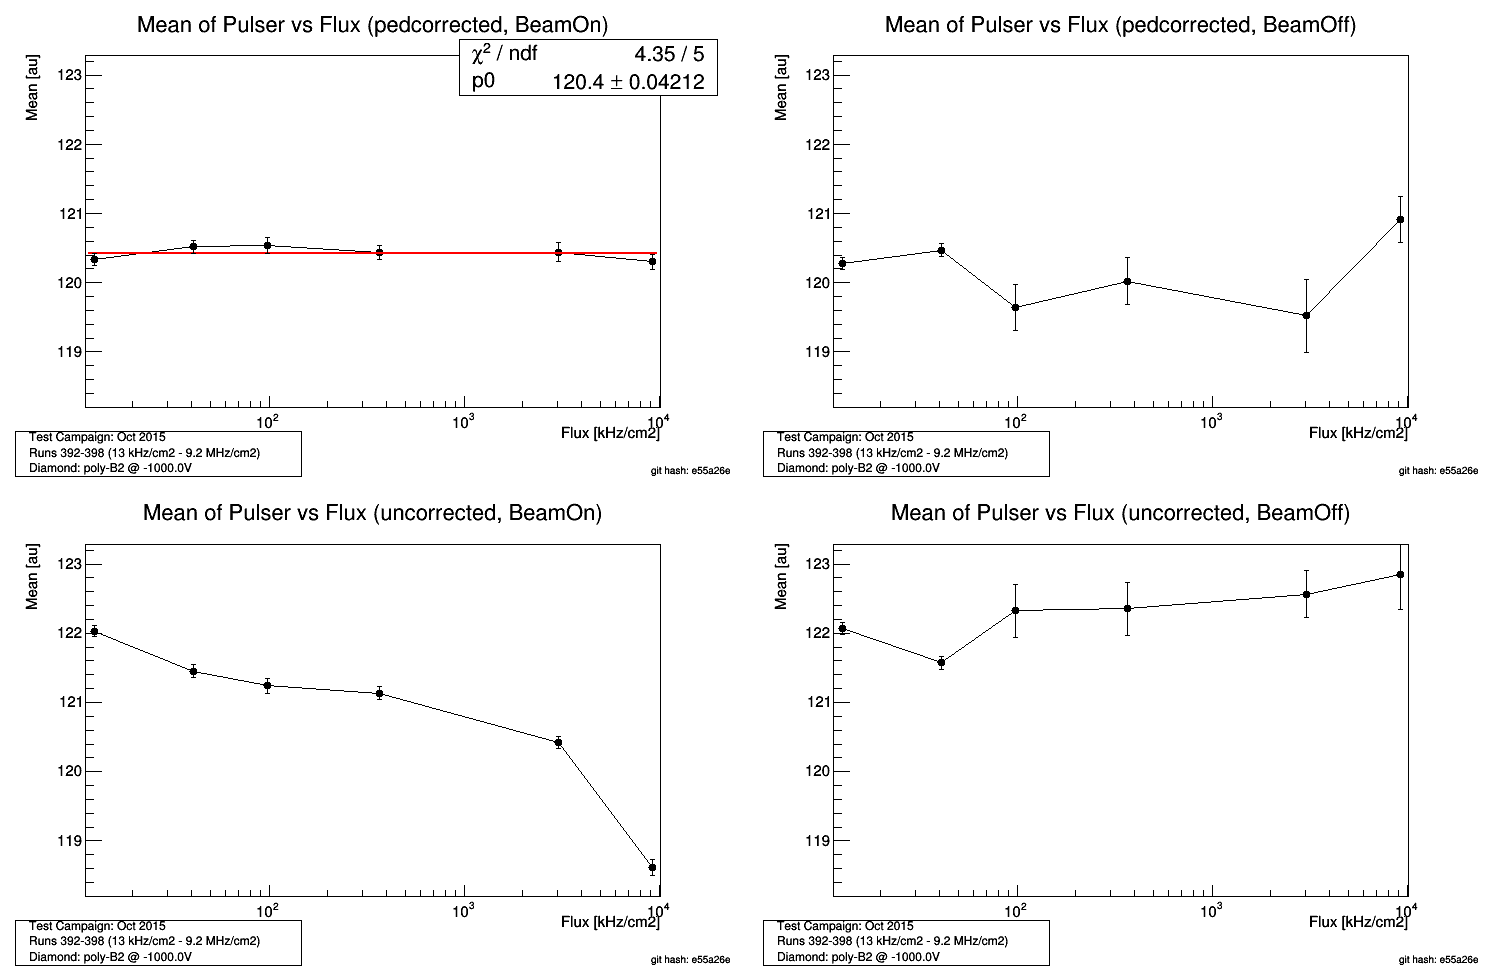
\includegraphics[width=10cm]{AllPulserOverviewMean0}
	\end{center}
\end{frame}
% ============================
\begin{frame}
	\begin{center}
		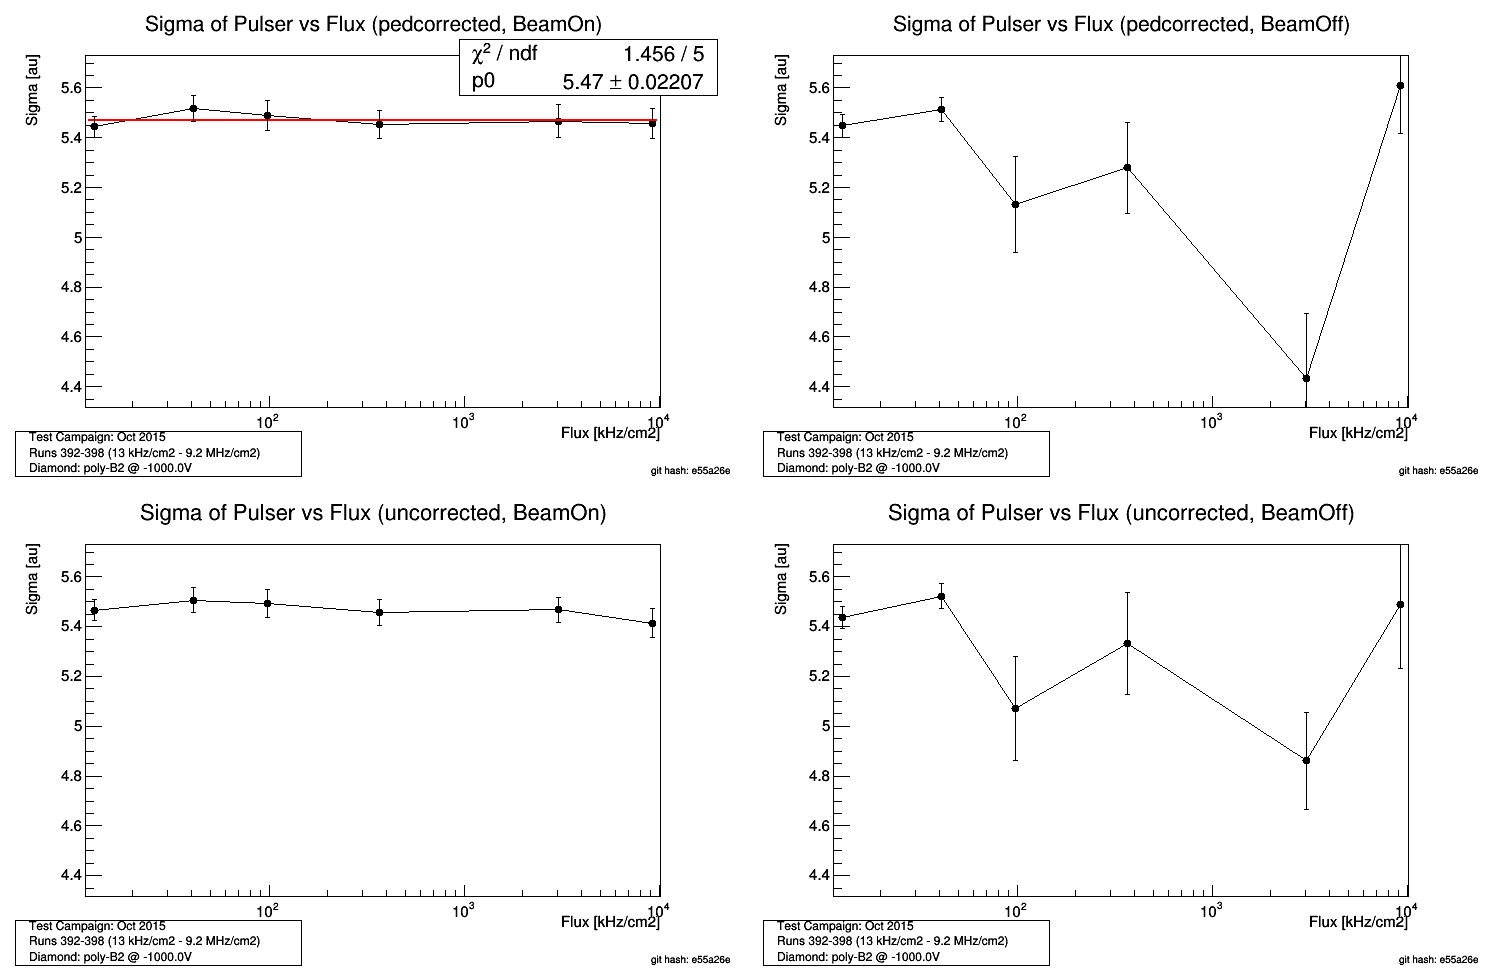
\includegraphics[width=10cm]{AllPulserOverviewSigma0}
	\end{center}
\end{frame}
% ============================
\begin{frame}
	\frametitle{Histograms}
	\begin{center}
		\begin{minipage}{5.5cm}
			\centering
			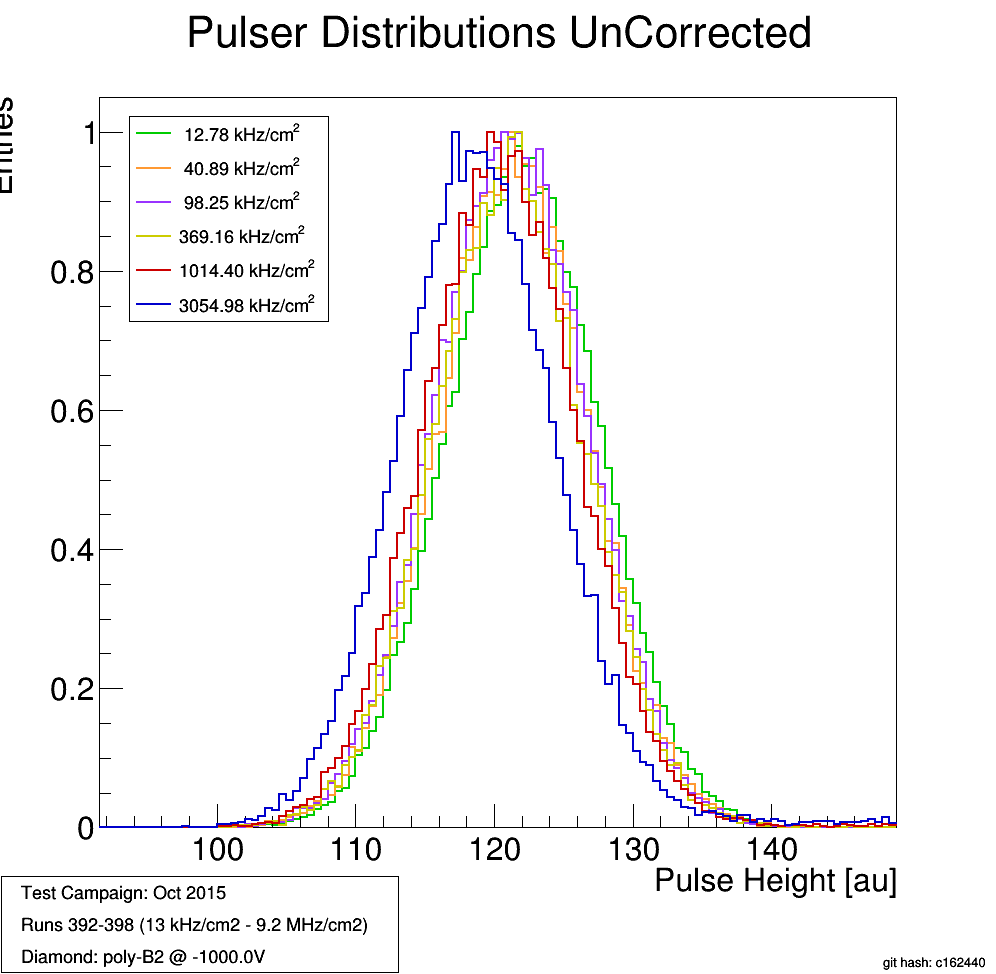
\includegraphics[width=5.2cm]{AllPulserHistosUncorrected0}\\
		\end{minipage}
		\begin{minipage}{5.5cm}
			\centering
			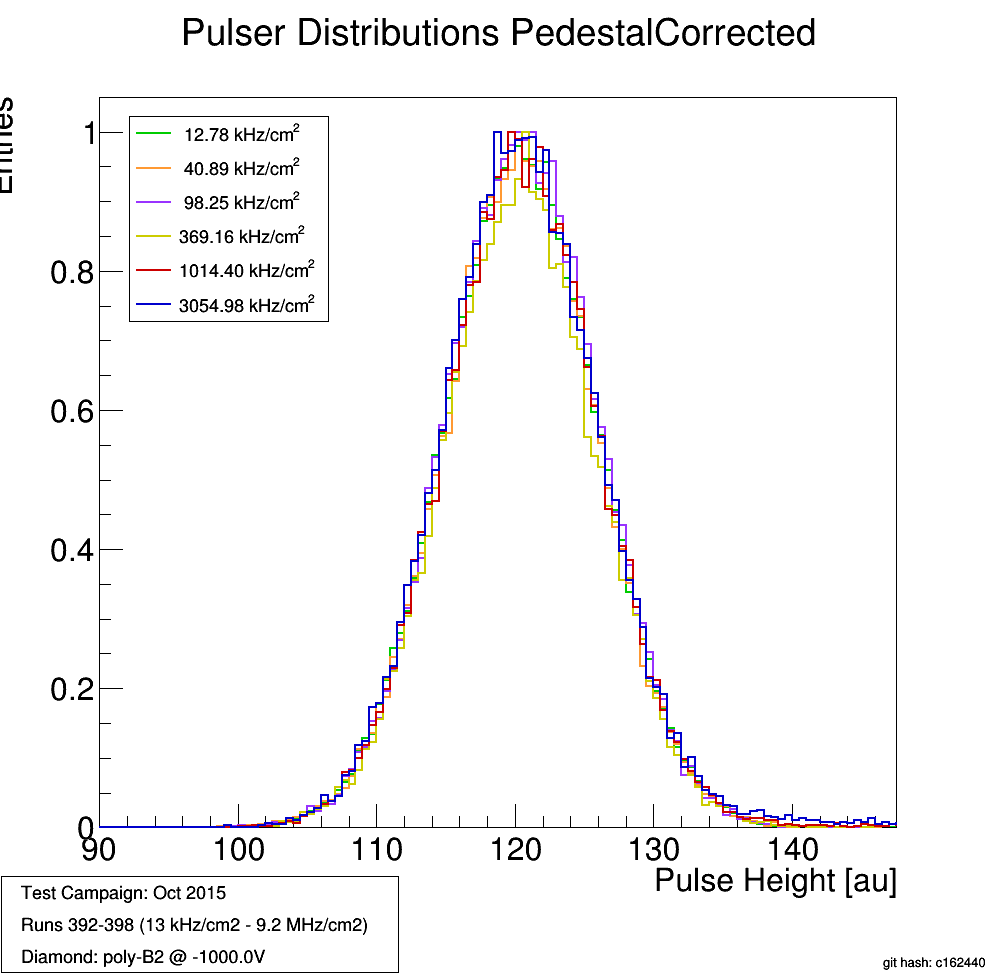
\includegraphics[width=5.2cm]{AllPulserHistos0}\\
		\end{minipage}
	\end{center}
\end{frame}
% ============================
\begin{frame}
	\frametitle{II6B2 pos}
	\begin{center}
		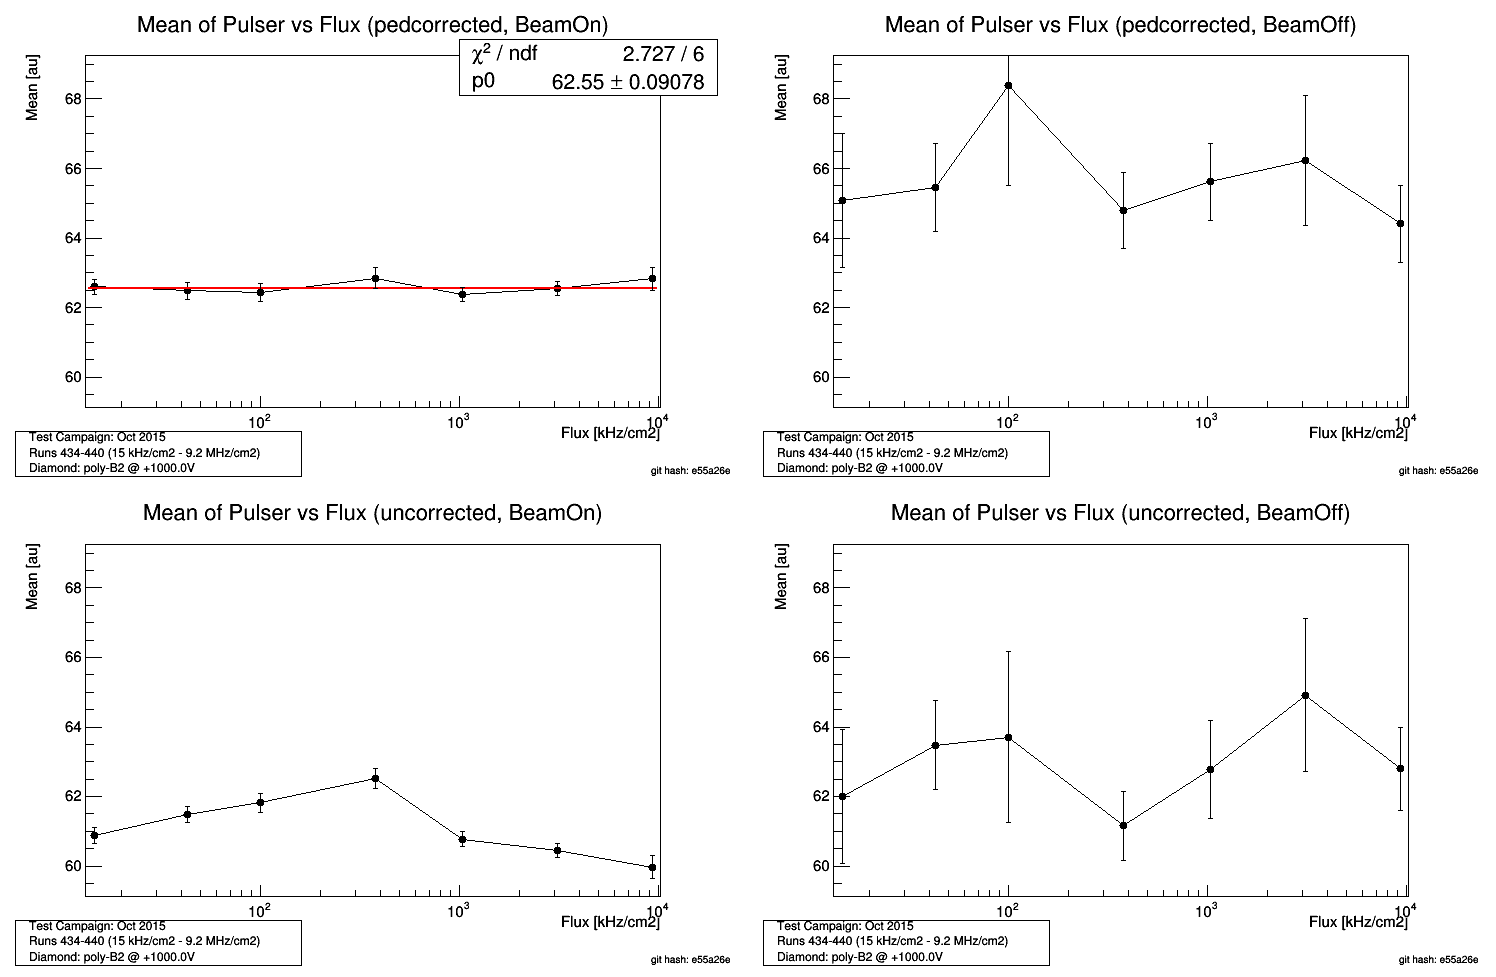
\includegraphics[width=10cm]{AllPulserOverviewMean3}
	\end{center}
\end{frame}
% ============================
\begin{frame}
	\begin{center}
		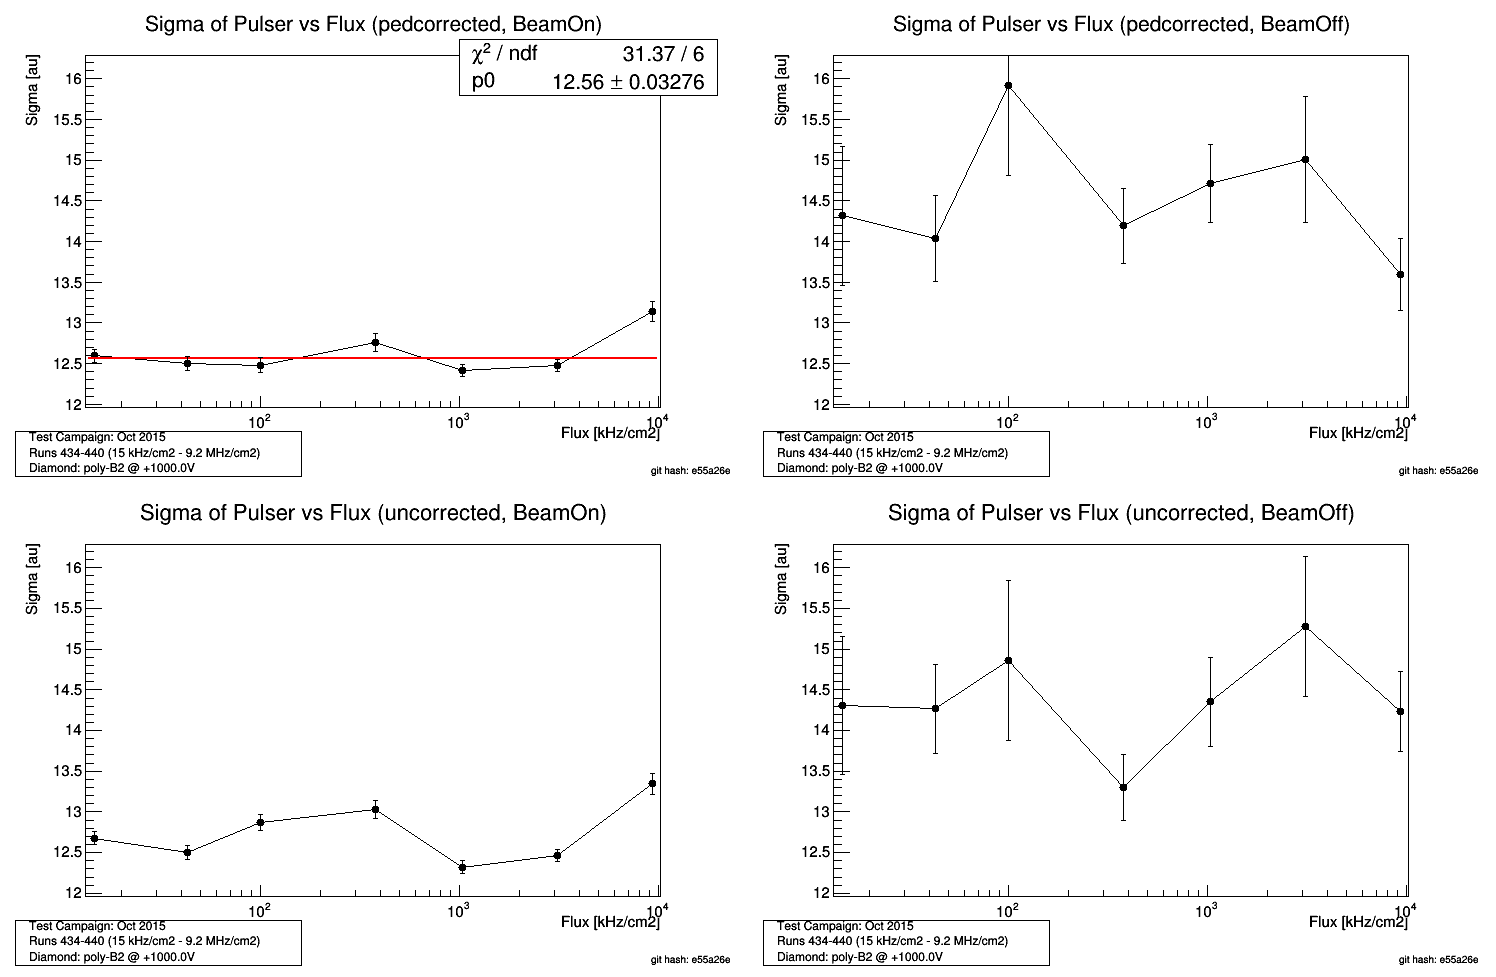
\includegraphics[width=10cm]{AllPulserOverviewSigma3}
	\end{center}
\end{frame}
% ============================
\begin{frame}
	\frametitle{S129 neg}
	\begin{center}
		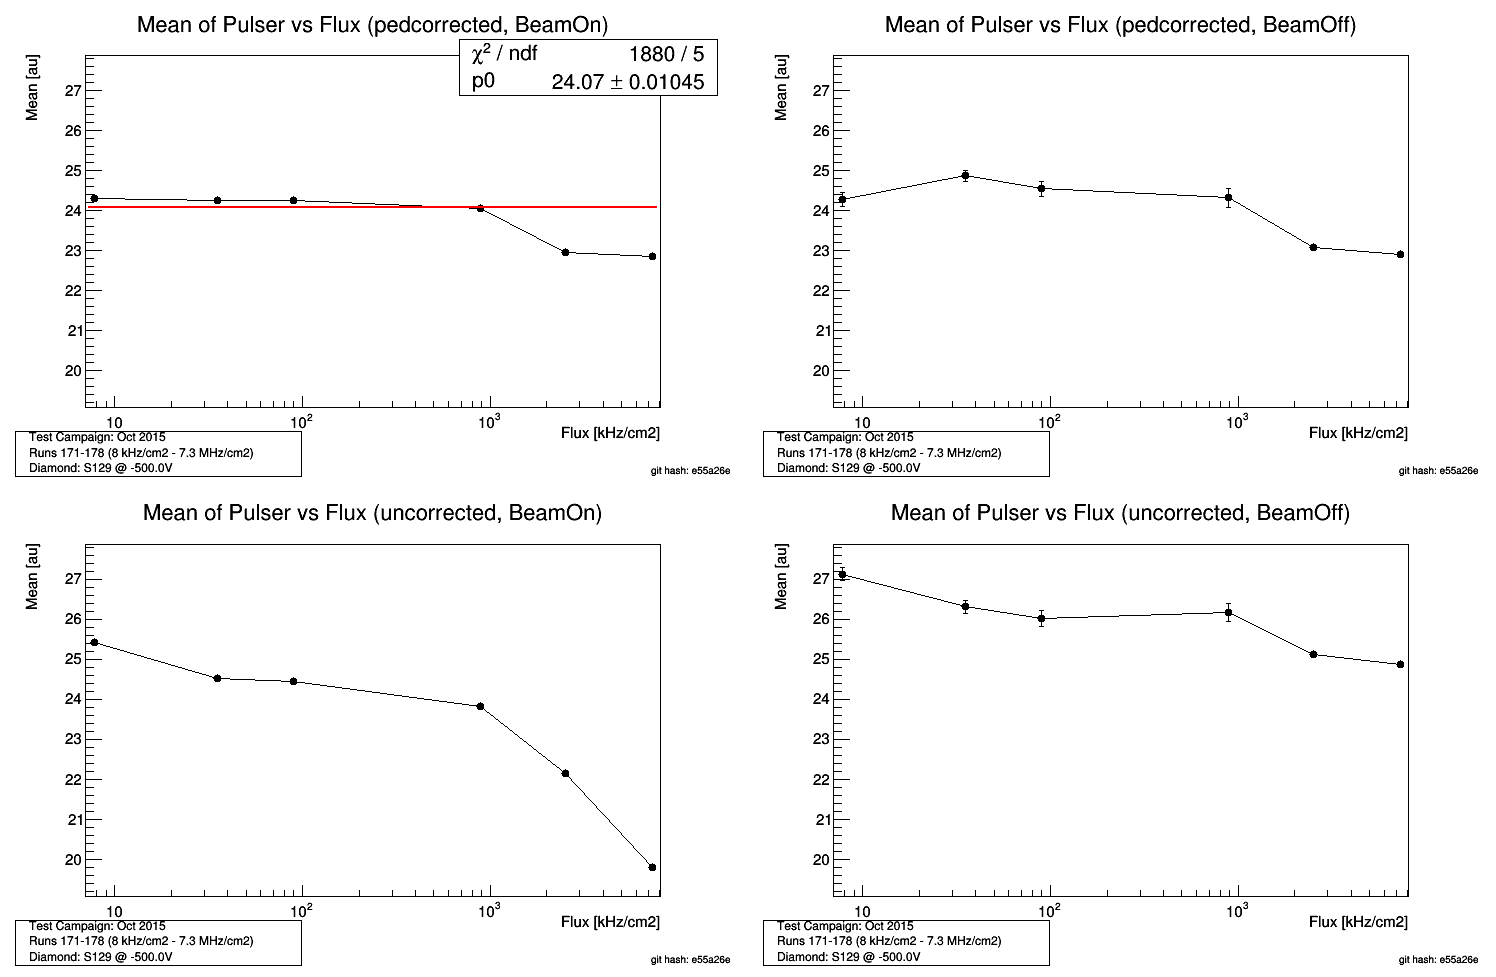
\includegraphics[width=10cm]{AllPulserOverviewMean1}
	\end{center}
\end{frame}
% ============================
\begin{frame}
	\begin{center}
		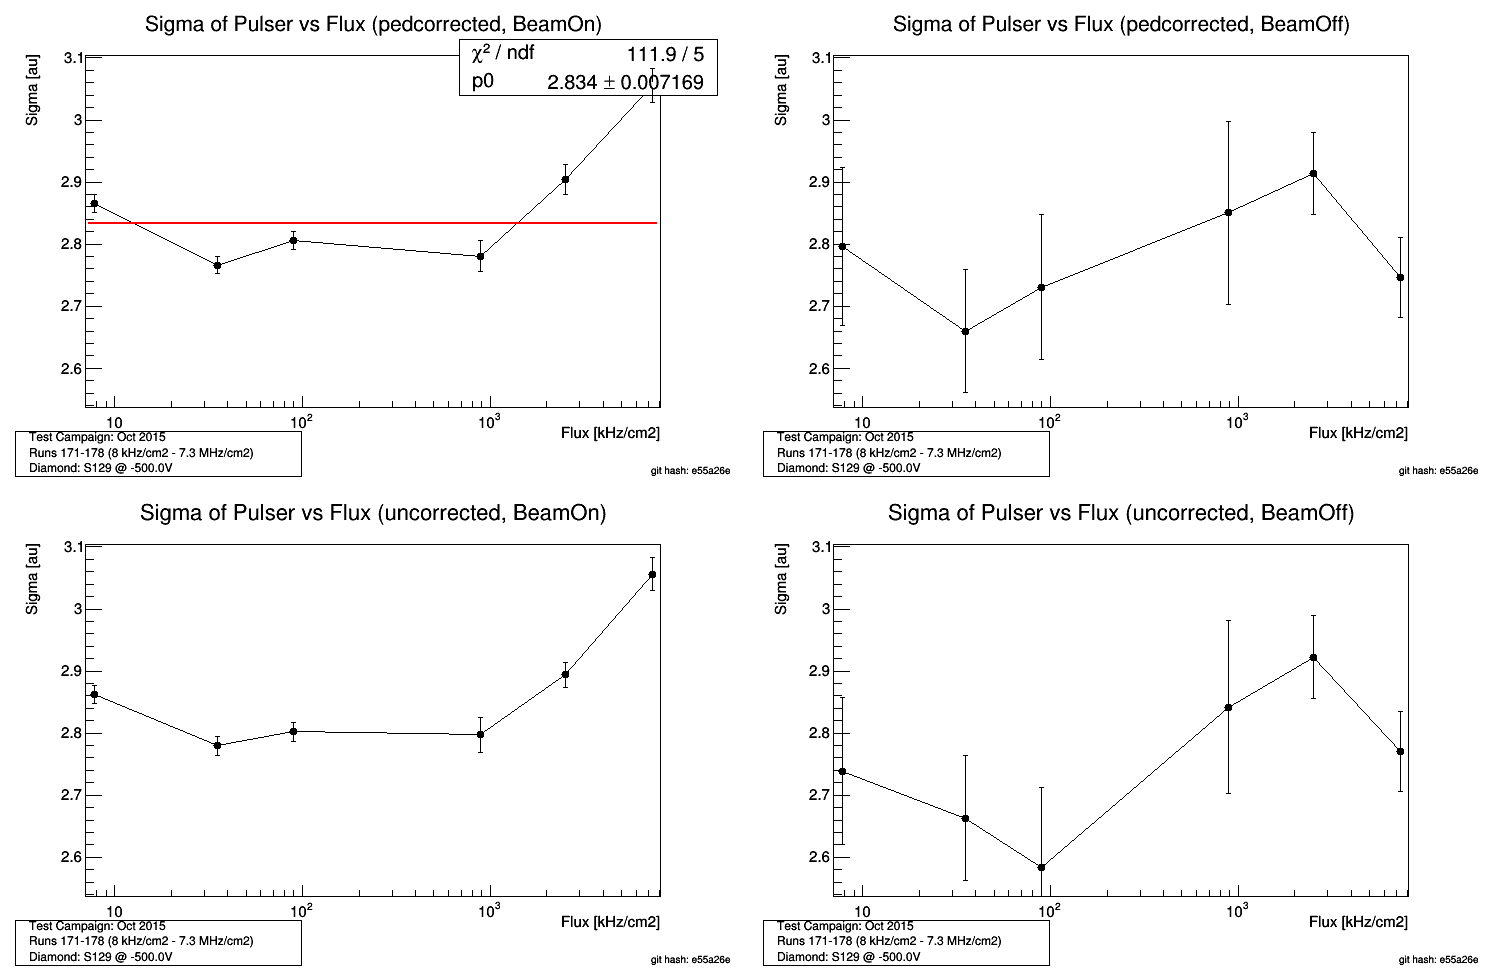
\includegraphics[width=10cm]{AllPulserOverviewSigma1}
	\end{center}
\end{frame}
% ============================
\begin{frame}
	\frametitle{Histograms}
	\begin{center}
		\begin{minipage}{5.5cm}
			\centering
			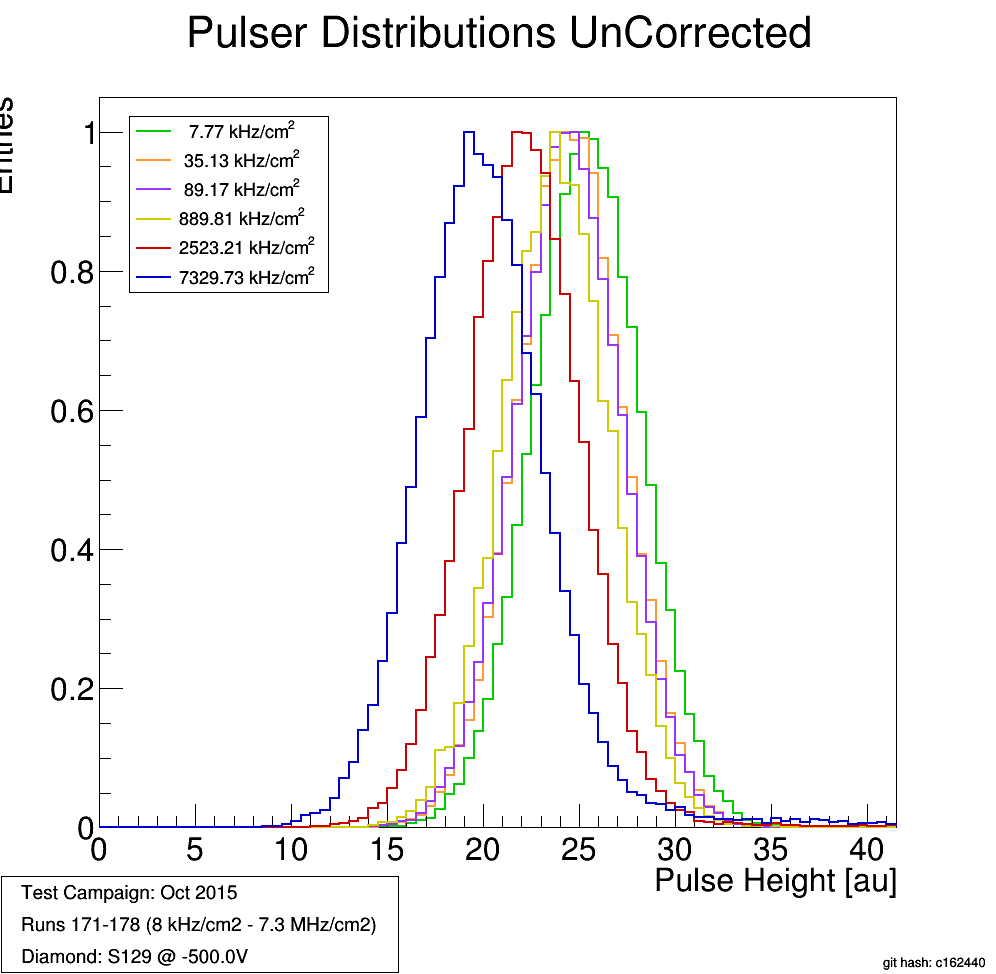
\includegraphics[width=5.2cm]{AllPulserHistosUncorrected1}\\
		\end{minipage}
		\begin{minipage}{5.5cm}
			\centering
			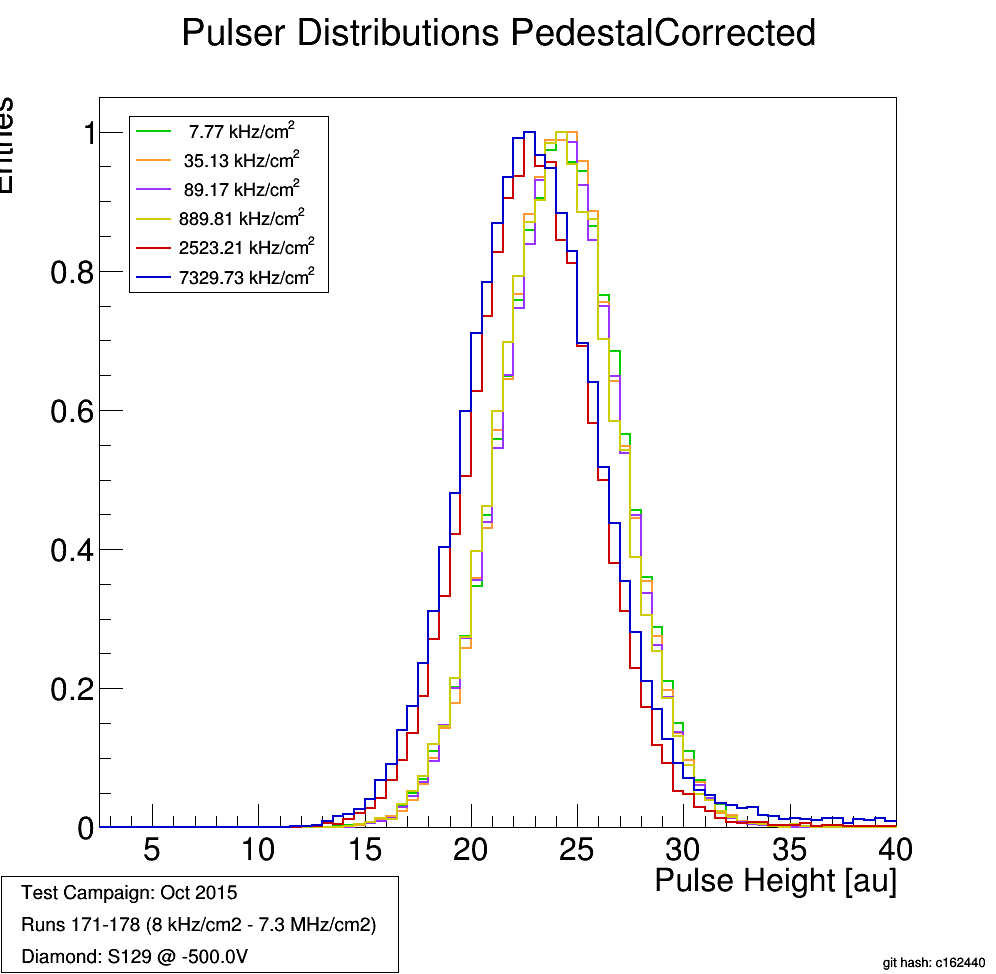
\includegraphics[width=5.2cm]{AllPulserHistos1}\\
		\end{minipage}
	\end{center}
\end{frame}
% ============================
\begin{frame}
	\frametitle{S129 pos}
	\begin{center}
		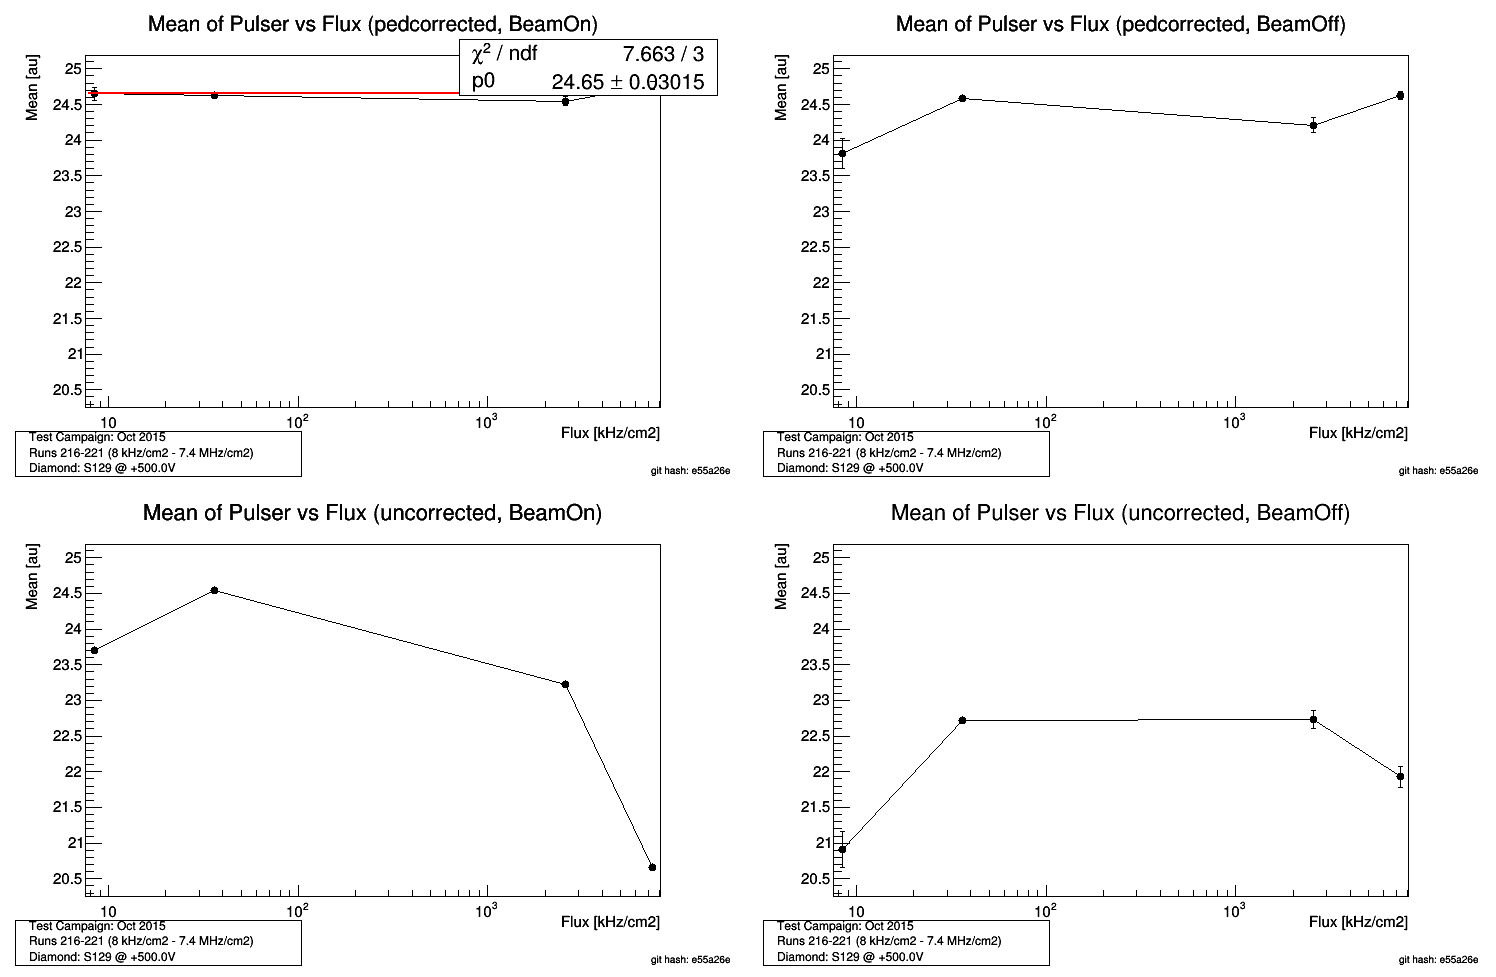
\includegraphics[width=10cm]{AllPulserOverviewMean2}
	\end{center}
\end{frame}
% ============================
\begin{frame}
	\begin{center}
		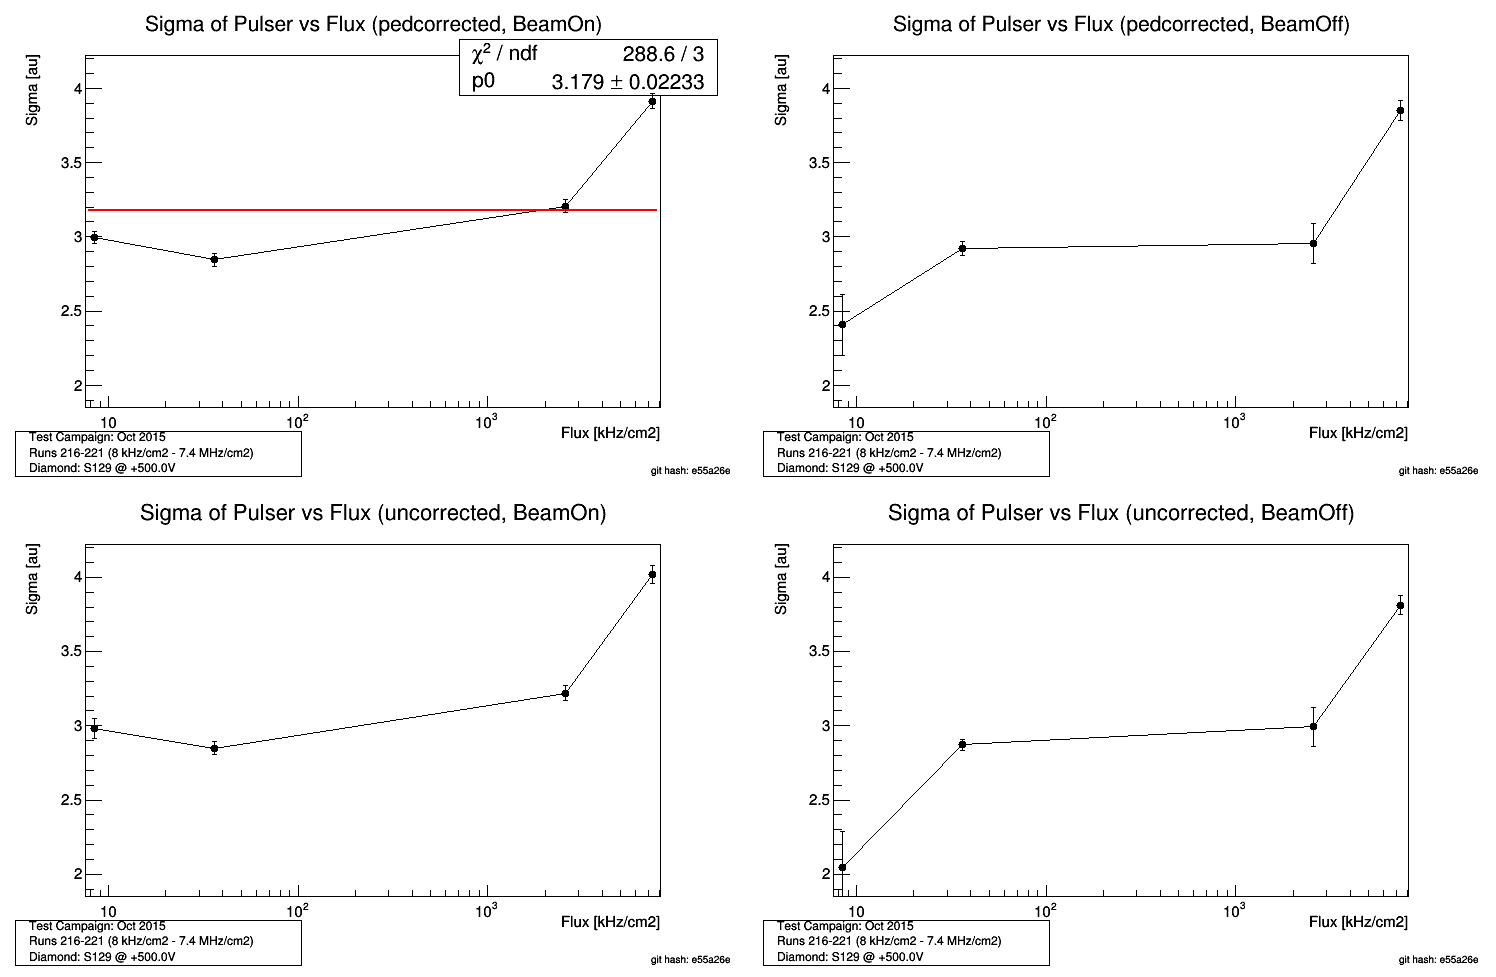
\includegraphics[width=10cm]{AllPulserOverviewSigma2}
	\end{center}
\end{frame}
% ============================
\begin{frame}
	\frametitle{Histograms}
	\begin{center}
		\begin{minipage}{5.5cm}
			\centering
			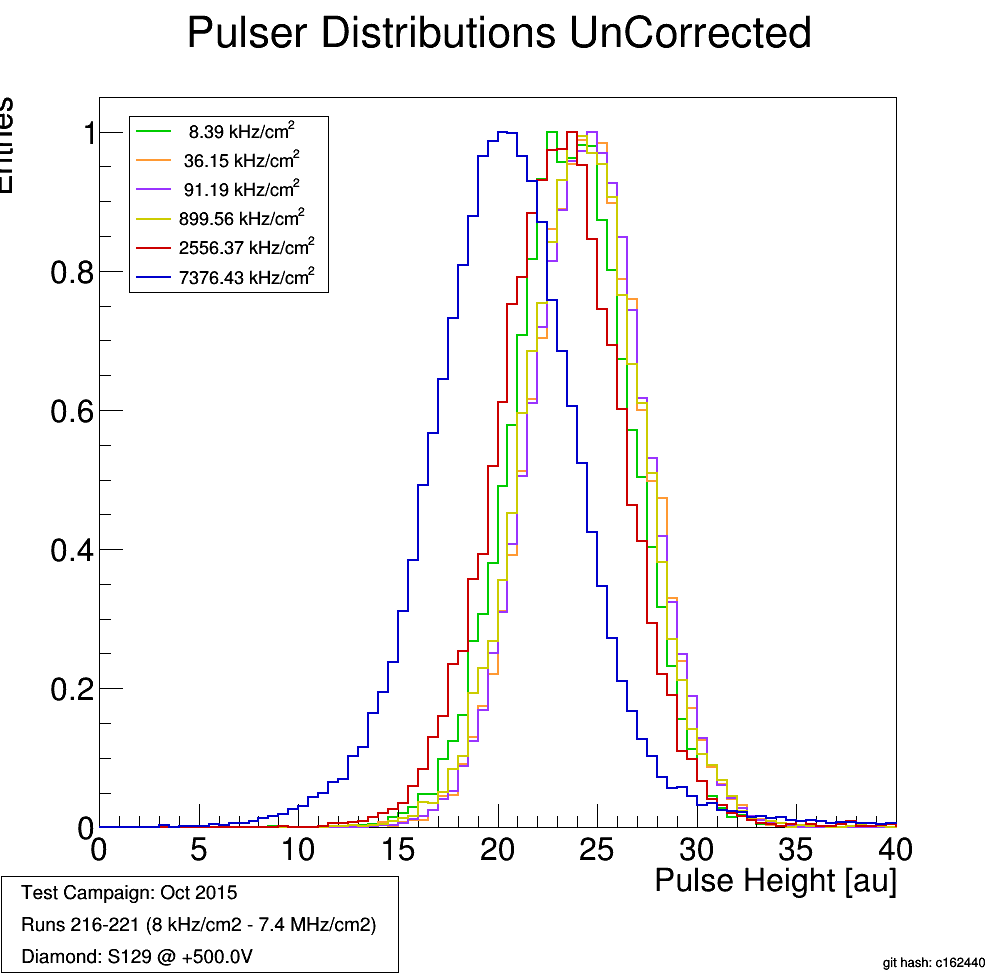
\includegraphics[width=5.2cm]{AllPulserHistosUncorrected2}\\
		\end{minipage}
		\begin{minipage}{5.5cm}
			\centering
			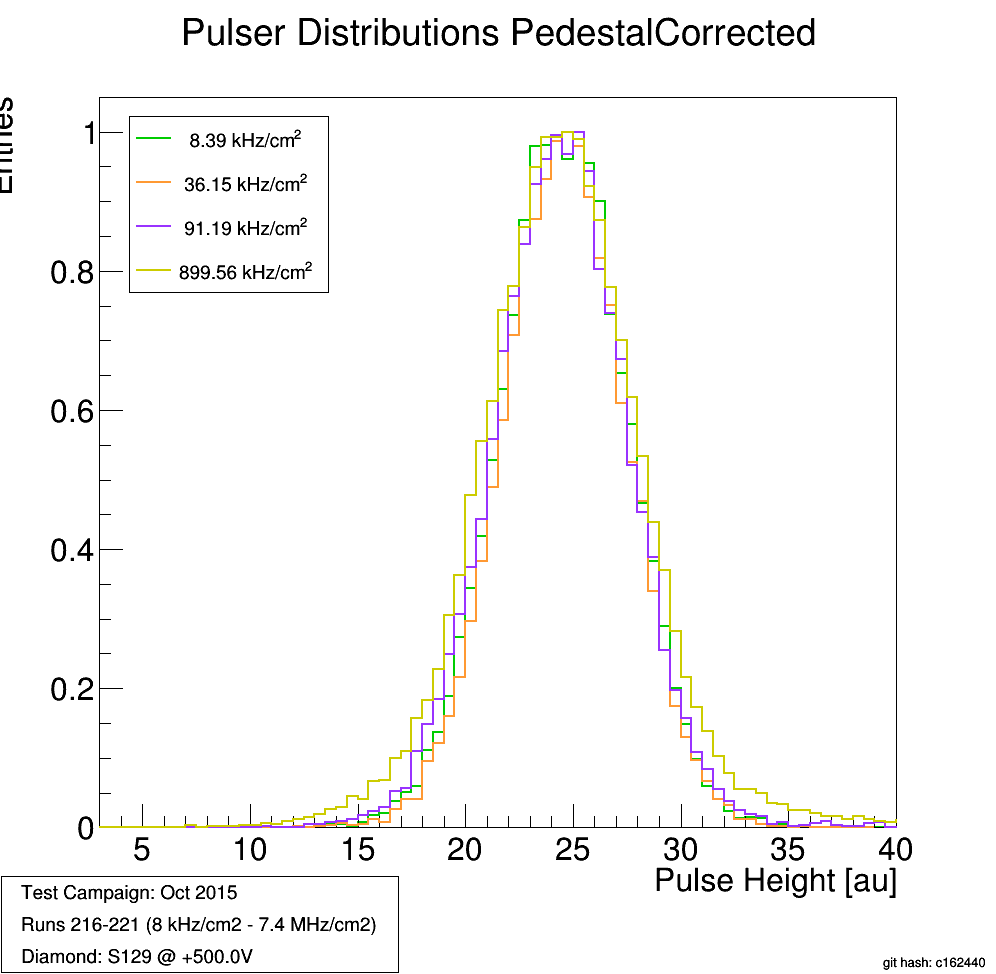
\includegraphics[width=5.2cm]{AllPulserHistos2}\\
		\end{minipage}
	\end{center}
\end{frame}
% ====================================================================================
\subsection{Pedestals}
\begin{frame}
	\frametitle{II6B2}
	\begin{center}
		\begin{minipage}{5.5cm}
			\centering
			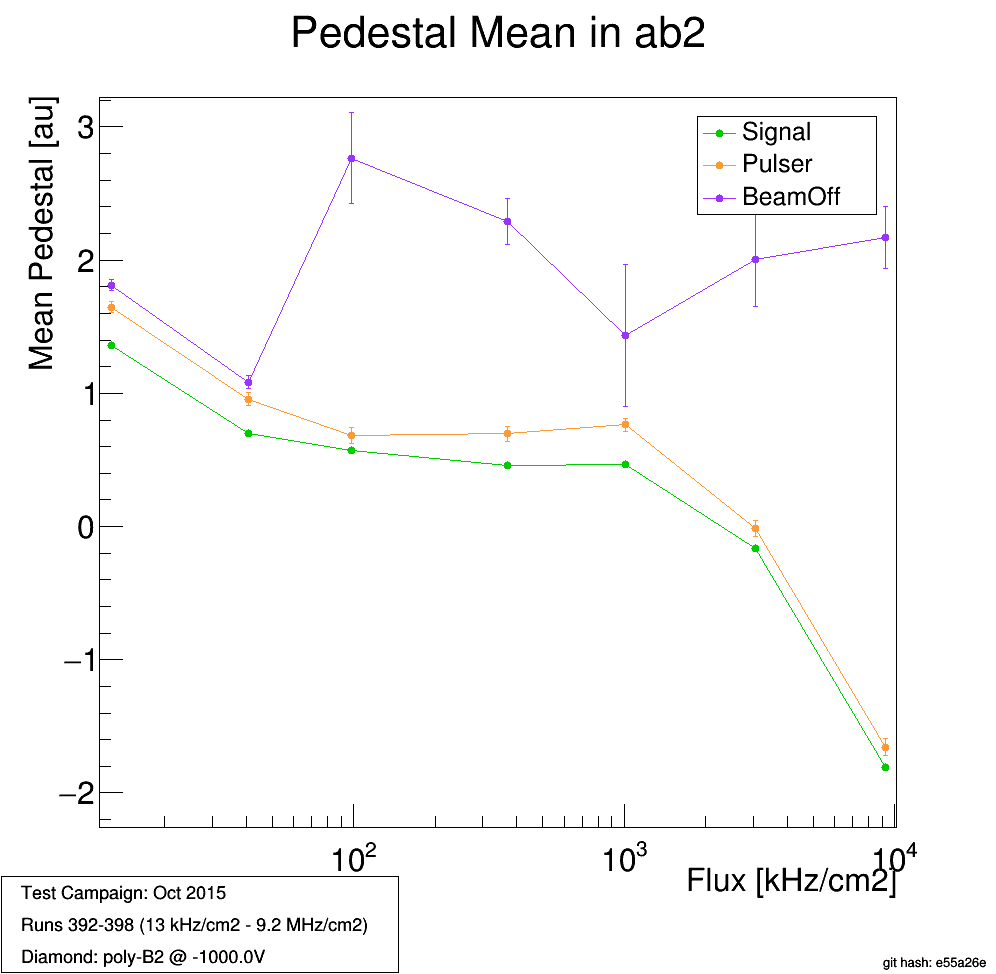
\includegraphics[width=5.2cm]{PulserPedestalComparison0}\\
		\end{minipage}
		\begin{minipage}{5.5cm}
			\centering
			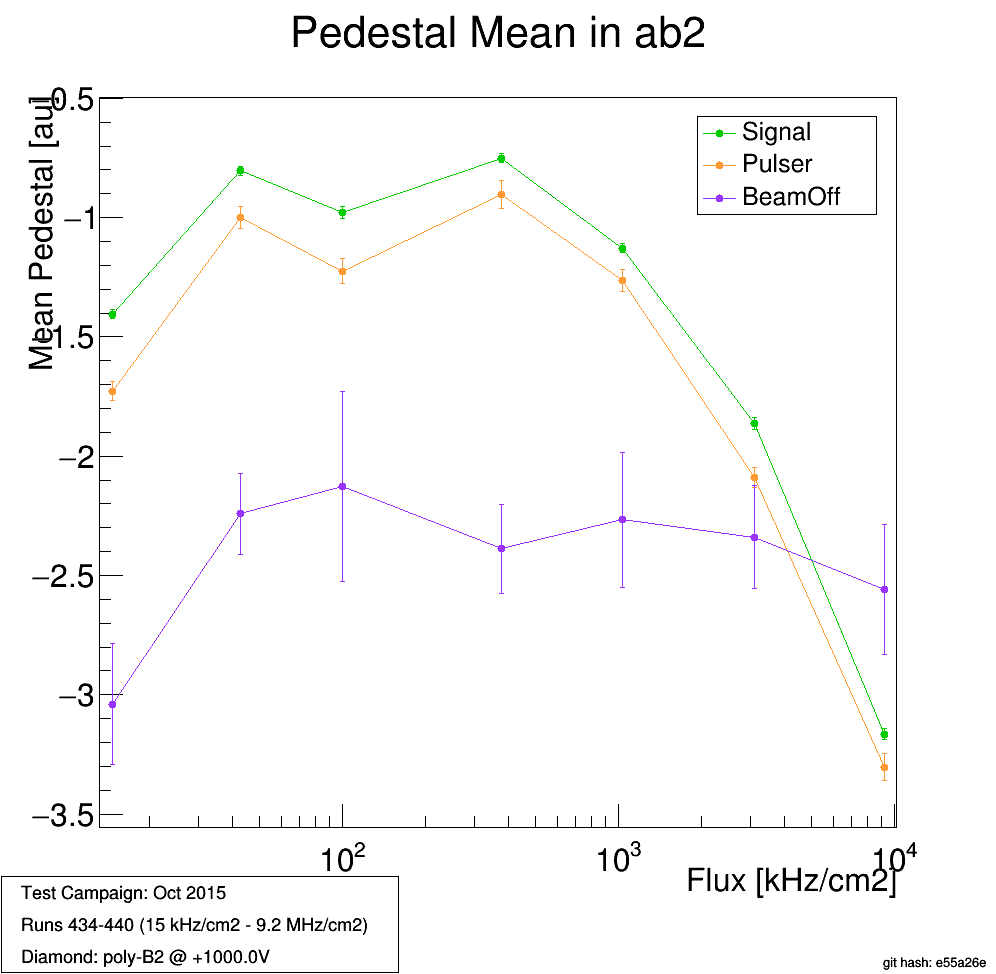
\includegraphics[width=5.2cm]{PulserPedestalComparison3}\\
		\end{minipage}
	\end{center}
\end{frame}
% ============================
\begin{frame}
	\frametitle{S129}
	\begin{center}
		\begin{minipage}{5.5cm}
			\centering
			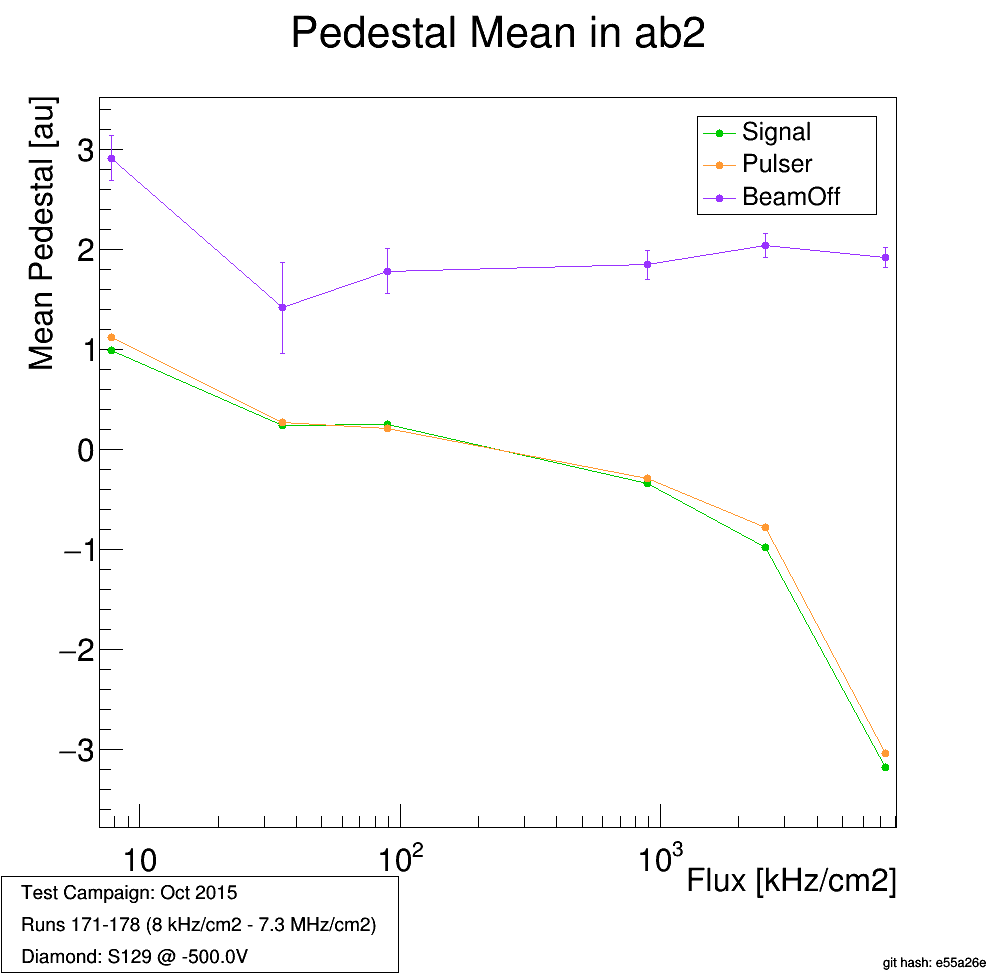
\includegraphics[width=5.2cm]{PulserPedestalComparison1}\\
		\end{minipage}
		\begin{minipage}{5.5cm}
			\centering
			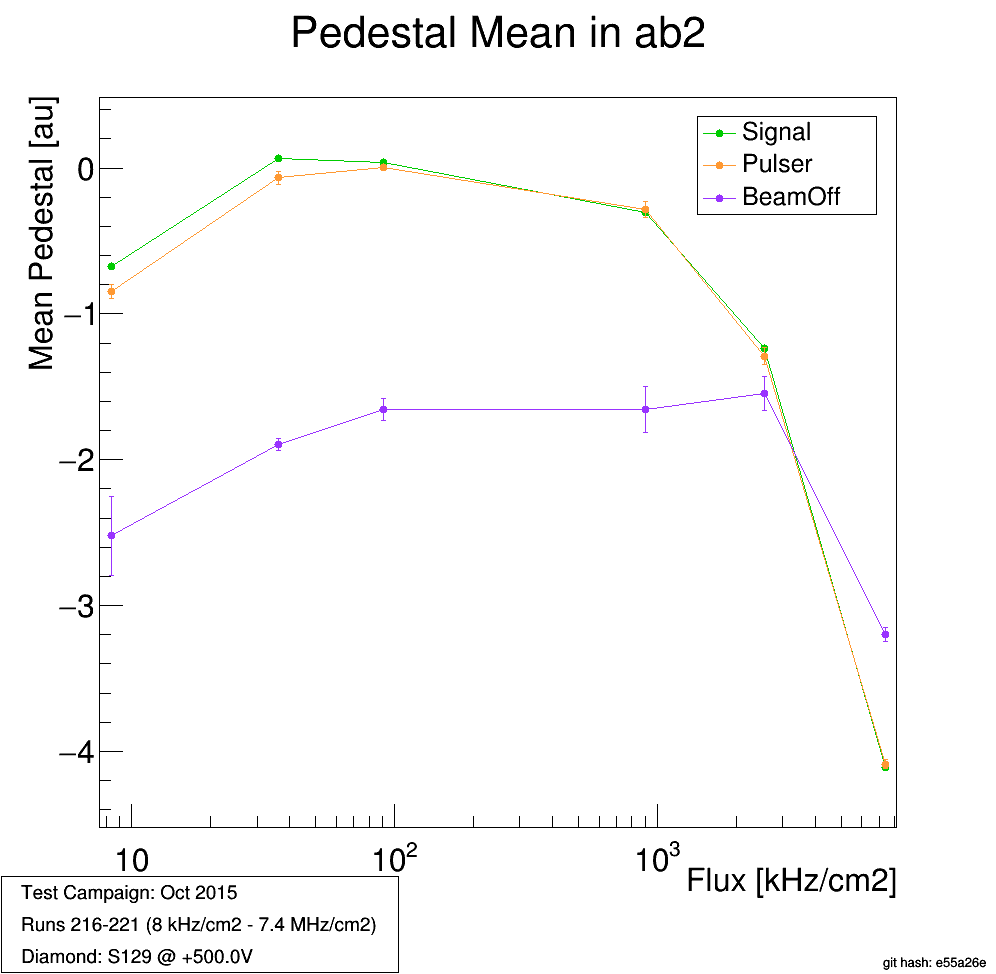
\includegraphics[width=5.2cm]{PulserPedestalComparison2}\\
		\end{minipage}
	\end{center}
\end{frame}
% ====================================================================================
\subsection{Pulse Heights}
\begin{frame}
	\frametitle{II6B2}
	\begin{center}
		\begin{minipage}{5.5cm}
			\centering
			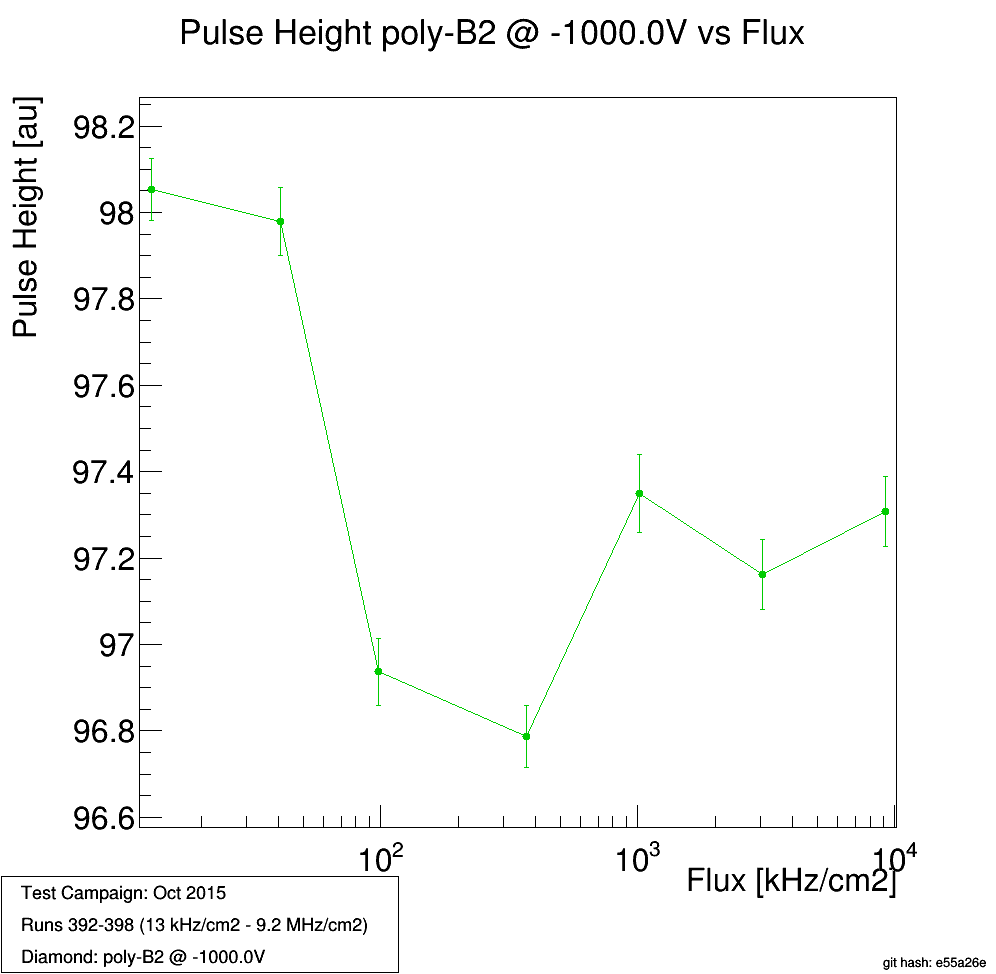
\includegraphics[width=5.2cm]{PulseHeightFlux0}\\
		\end{minipage}
		\begin{minipage}{5.5cm}
			\centering
			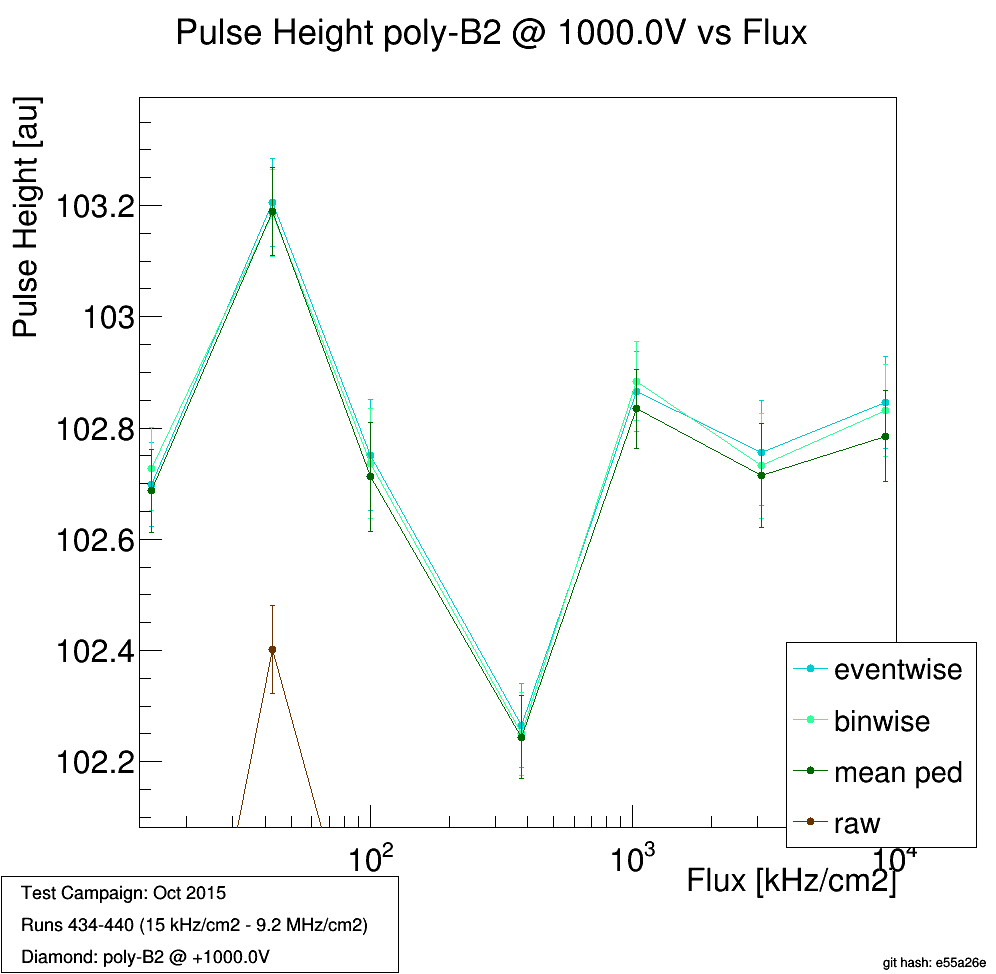
\includegraphics[width=5.2cm]{PulseHeightFlux1}\\
		\end{minipage}
	\end{center}
\end{frame}
% ============================
\begin{frame}
	\frametitle{II6B2}
	\begin{center}
		\begin{minipage}{5.5cm}
			\centering
			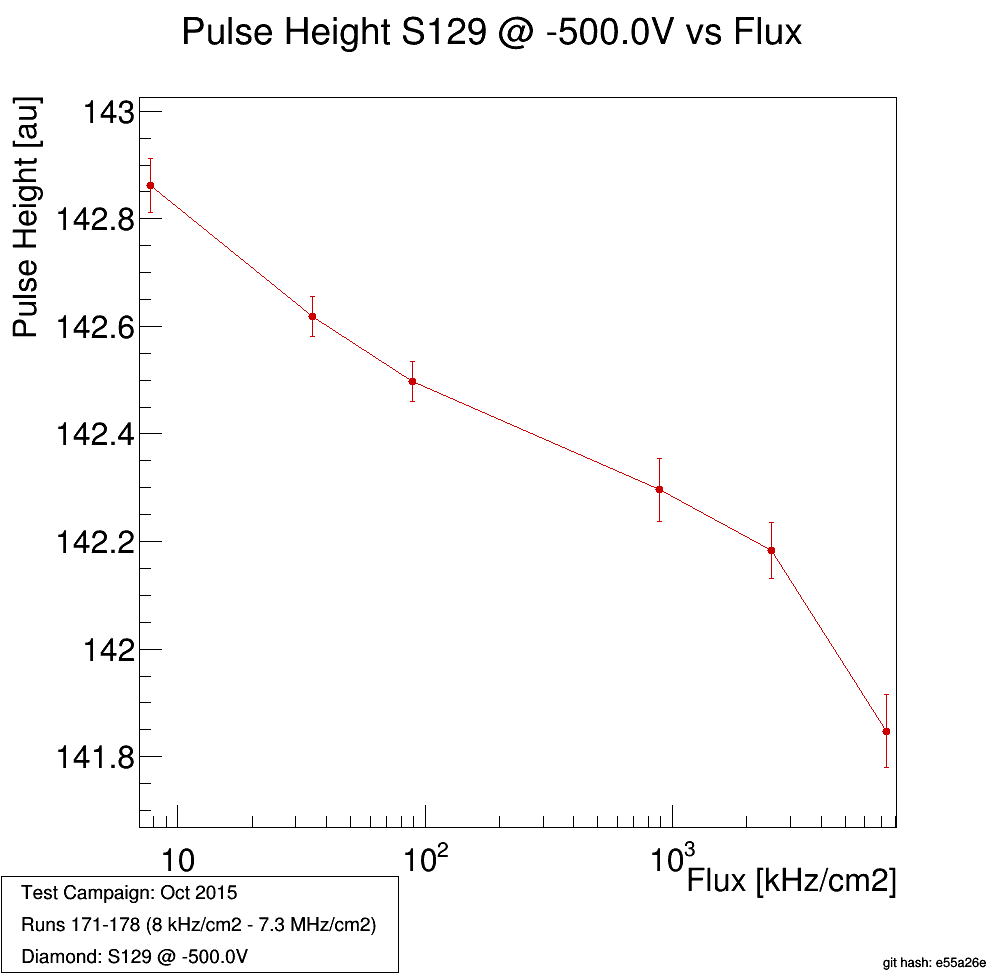
\includegraphics[width=5.2cm]{PulseHeightFlux2}\\
		\end{minipage}
		\begin{minipage}{5.5cm}
			\centering
			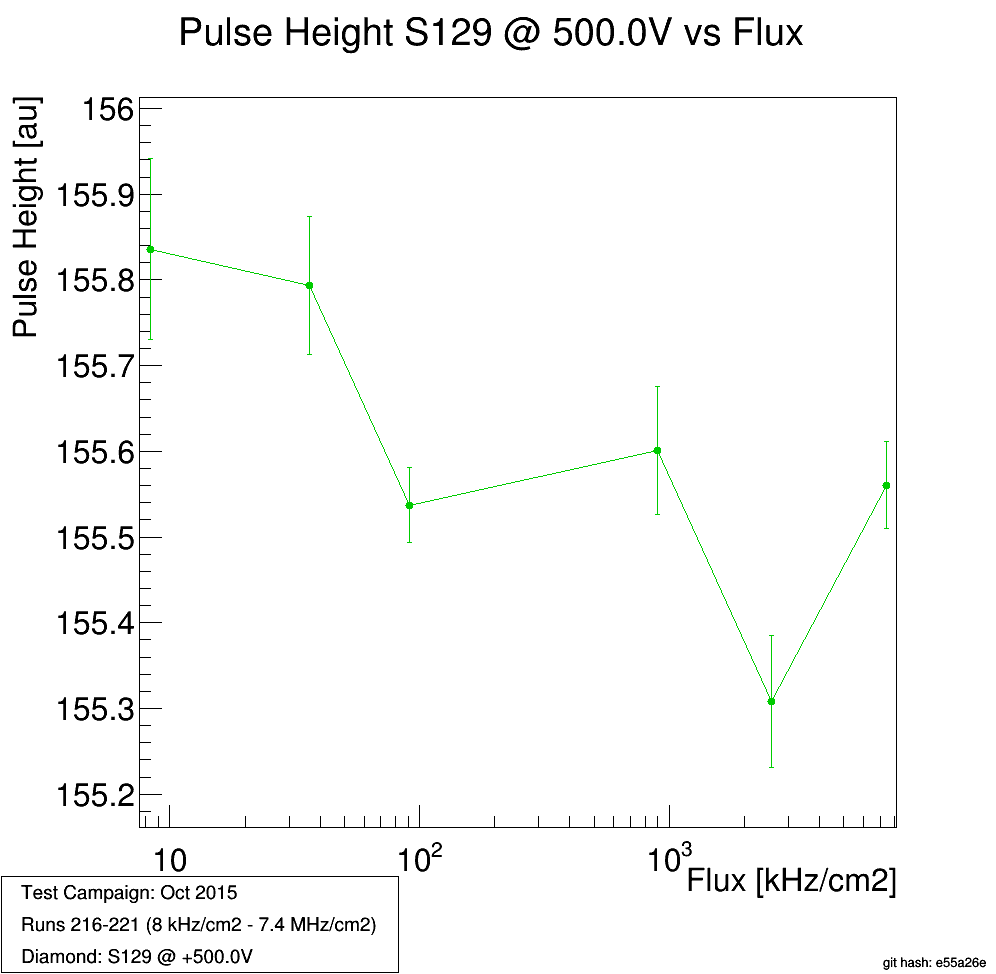
\includegraphics[width=5.2cm]{PulseHeightFlux3}\\
		\end{minipage}
	\end{center}
\end{frame}
% ====================================================================================
% PULSER
% ====================================================================================
\section{Conclusion}
% ============================
\begin{frame}
	\frametitle{Conclusion}
	\begin{itemize}
		\setlength{\itemsep}{\fill}	
		\item measurements with two different pulsers:
			\begin{itemize}
				\item internal
				\item external
			\end{itemize}
		\item poly has wider distribution

	\end{itemize}
\end{frame}

% ============================
% DOCUMENT END
\end{document}

